% Question  ##################################################################################################################
\section{Question 3}\label{ssec:pt2q3}
\textbf{Hidden Markov Models (HMM) are an important unsupervised learning method used to analyse sequence data and identifying underlying regimes that govern the data.}

\noindent
\textbf{This question relates to detecting regime changes in volatility (risk).}
% END Question  ##############################################################################################################

% Question (i) ###############################################################################################################
\subsection{Q2 (i)}\label{sssec:pt2q3i}
\textbf{Download and calculate the last 10 year daily returns of the S\&P500 index (till 31/12/2017).}

\noindent
Code to download the closing prices for S\&P500 in this question can be found in ‘Question 3 (i)’ in the python notebook. The data was downloaded from Yahoo Finance and saved as .csv format in the following path \textit{‘src/data/part\_2’}. The file was saved as \textit{‘GSPC.csv’}. The data was then reloaded from the file and converted into pandas dataframe and the daily log returns were computed.
% END Question (i) ###########################################################################################################

% Question (ii) ##############################################################################################################
\subsection{Q2 (ii)}\label{sssec:pt2q3ii}
\textbf{Create a new series of volatility based on 10 day rolling time window (for each day apply standard deviation on the previous 10 day returns).}

\noindent
To calculate the 10 day rolling volatility a function called 'rolling\_vol' was created in the 'fintech' library as shown in Fig.~\ref{fig:rollvol}, and this was called from the notebook in 'Question 3 (ii)'. 

\begin{figure}[H]
\centering
  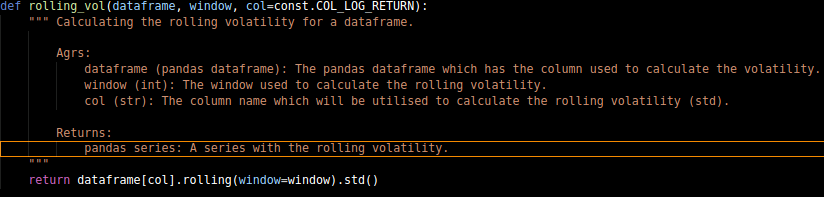
\includegraphics[scale = .58]{imgs/rolling_vol.png}
  \caption{Function to calculate rolling volatility.}
  \label{fig:rollvol}
\end{figure}
% END Question (ii) ##########################################################################################################

% Question (iii) ############################################################################################################

\subsection{Q2 (iii)}\label{sssec:pt2q3iii}
\textbf{Utilize this new series to train two Gaussian HMM: one using 2 latent states and the other with 3 latent states (components).  These latent states indicate the different volatility regimes.}

\noindent
The code to train the two models can be found in 'Question 3 (iii)'. Both models were trained using 1000 iteration using a diagonal covariance matrix. Also both models were trained using one feature, which is the series created in (ii). A third party library called 'hmmlearn' \cite{python:hmmlearn} was utilised for this task. 

% END Question (iii) #########################################################################################################

% Question (iv) ##############################################################################################################

\subsection{Q2 (iv)}\label{sssec:pt2q3iv}
\textbf{For each of the two models above, present a visualization (one or more plots) which clearly shows the identified volatility regimes over the 10-year period being investigated.}

\noindent
Fig.~\ref{fig:regime1} shows the volatility regime over the 10-period when using 2 latent states while Fig.~\ref{fig:regime2} shows the volatility regimes when using 3 latent states. The code for these plots can be found in the notebook in 'Question 3 (iv)'.

\begin{figure}[H]
\centering
  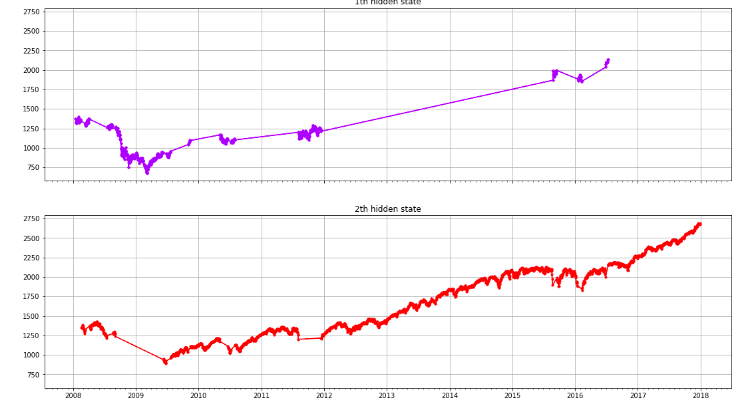
\includegraphics[scale = .60]{imgs/regime1.png}
  \caption{Volatility regime over the 10-period when using 2 latent states.}
  \label{fig:regime1}
\end{figure}

\begin{figure}[H]
\centering
  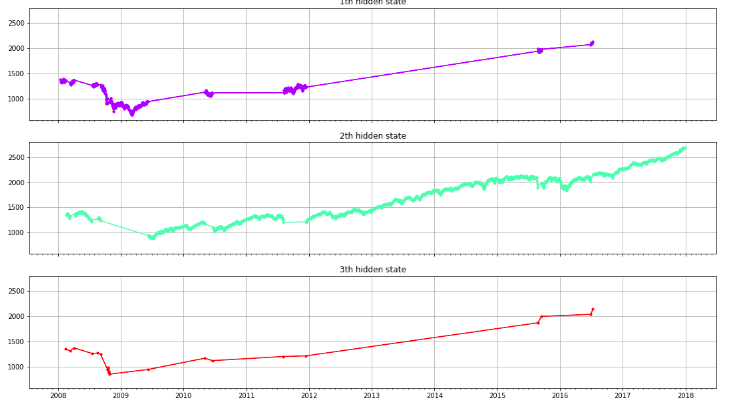
\includegraphics[scale = .65]{imgs/regime2.png}
  \caption{Volatility regime over the 10-period when using 3 latent states.}
  \label{fig:regime2}
\end{figure}

% END Question (iv) ##########################################################################################################

% Question (v) ###############################################################################################################

\subsection{Q2 (v)}\label{sssec:pt2q3v}
\textbf{Comment on the findings and discuss the difference in outcomes between the two models.}

\noindent
Using the models in the previous question (iii) the Hidden Markov model enables us to investigate underlying latent states (must specify the number of components in this unsupervised learning model) and the probability transitions between them even though they are not directly observable. 

\noindent
Finding volatility regimes can help an investor to manage risk more effectively by identifying states where there is high volatility. This model has the potential of identifying incorrect identification of a “trend”. 

\noindent 
As seen from both the plots the regime detection captures highly volatile and “trending” periods. In the first model (two latent states) the majority is captured in the 2nd state but most of 2008-2009 and late 2011 is captured in the first state. In the second model the majority was captured in the 2nd state, while most of 2008-2009 was captured in the first state together with the late 2011 period. Utilizing these regimes one can apply different investing/risk management methods according to the state the asset is in, in terms of volatility. The states which were captured show a low volatility state and a high volatility state/s.

\noindent
All the states in the two models have a positive mean. The variance of the 2nd state in both models indicate low variance (low volatility periods), but the first state has a variance which is significantly higher in both models (high volatility periods). This indicates a state with high volatility. The third state in the second model also indicate high volatility but it must be noted that this state captures relatively low information. 

\noindent
It is also important to note the states during the 2008 period (market crash), as you can see both models captured high volatility during that period (both models capture this in the first state). The measurements discussed above (mean and var) are shown in Fig.~\ref{fig:model_a_regime} and Fig.~\ref{fig:model_b_regime}. 

\begin{figure}[H]
     \centering
     \begin{subfigure}[b]{0.45\textwidth}
         \centering
         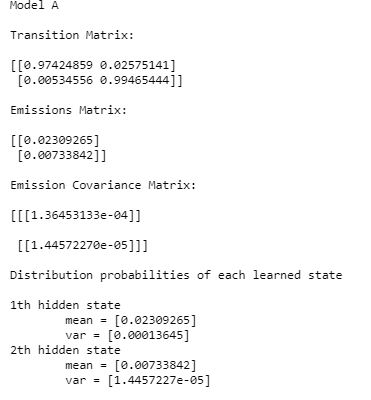
\includegraphics[width=\textwidth]{imgs/model_a_regime.JPG}
         \caption{HMM measurements for Model A (two latent states).}
         \label{fig:model_a_regime}
     \end{subfigure}
     \hfill
     \begin{subfigure}[b]{0.45\textwidth}
         \centering
                 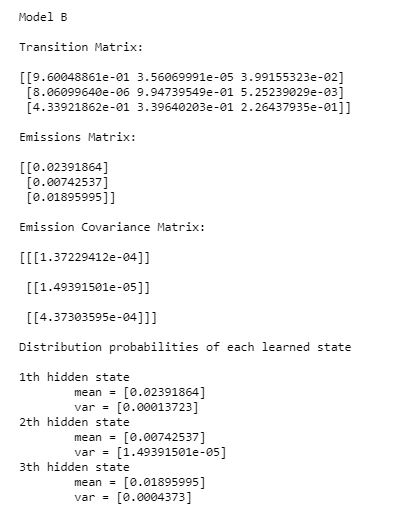
\includegraphics[width=\textwidth]{imgs/model_b_regime.JPG}
        \caption{HMM measurements for Model B (three latent states).}
         \label{fig:model_b_regime}
     \end{subfigure}
\end{figure}


% END Question (v) ###########################################################################################################

